\UseRawInputEncoding
\documentclass[12pt]{article}
\title{ECE 141 Homework 2}
\usepackage{subcaption}
\author{Lawrence Liu}
\usepackage{graphicx}
\usepackage{amsmath}
\usepackage{placeins}
\newcommand{\Laplace}{\mathscr{L}}
\setlength{\parskip}{\baselineskip}%
\setlength{\parindent}{0pt}%
\usepackage{xcolor}
\usepackage{listings}
\definecolor{backcolour}{rgb}{0.95,0.95,0.92}
\usepackage{amssymb}
\lstdefinestyle{mystyle}{
    backgroundcolor=\color{backcolour}}
\lstset{style=mystyle}

\begin{document}
\maketitle
\section*{Problem 3.21}
\subsection*{(a)}
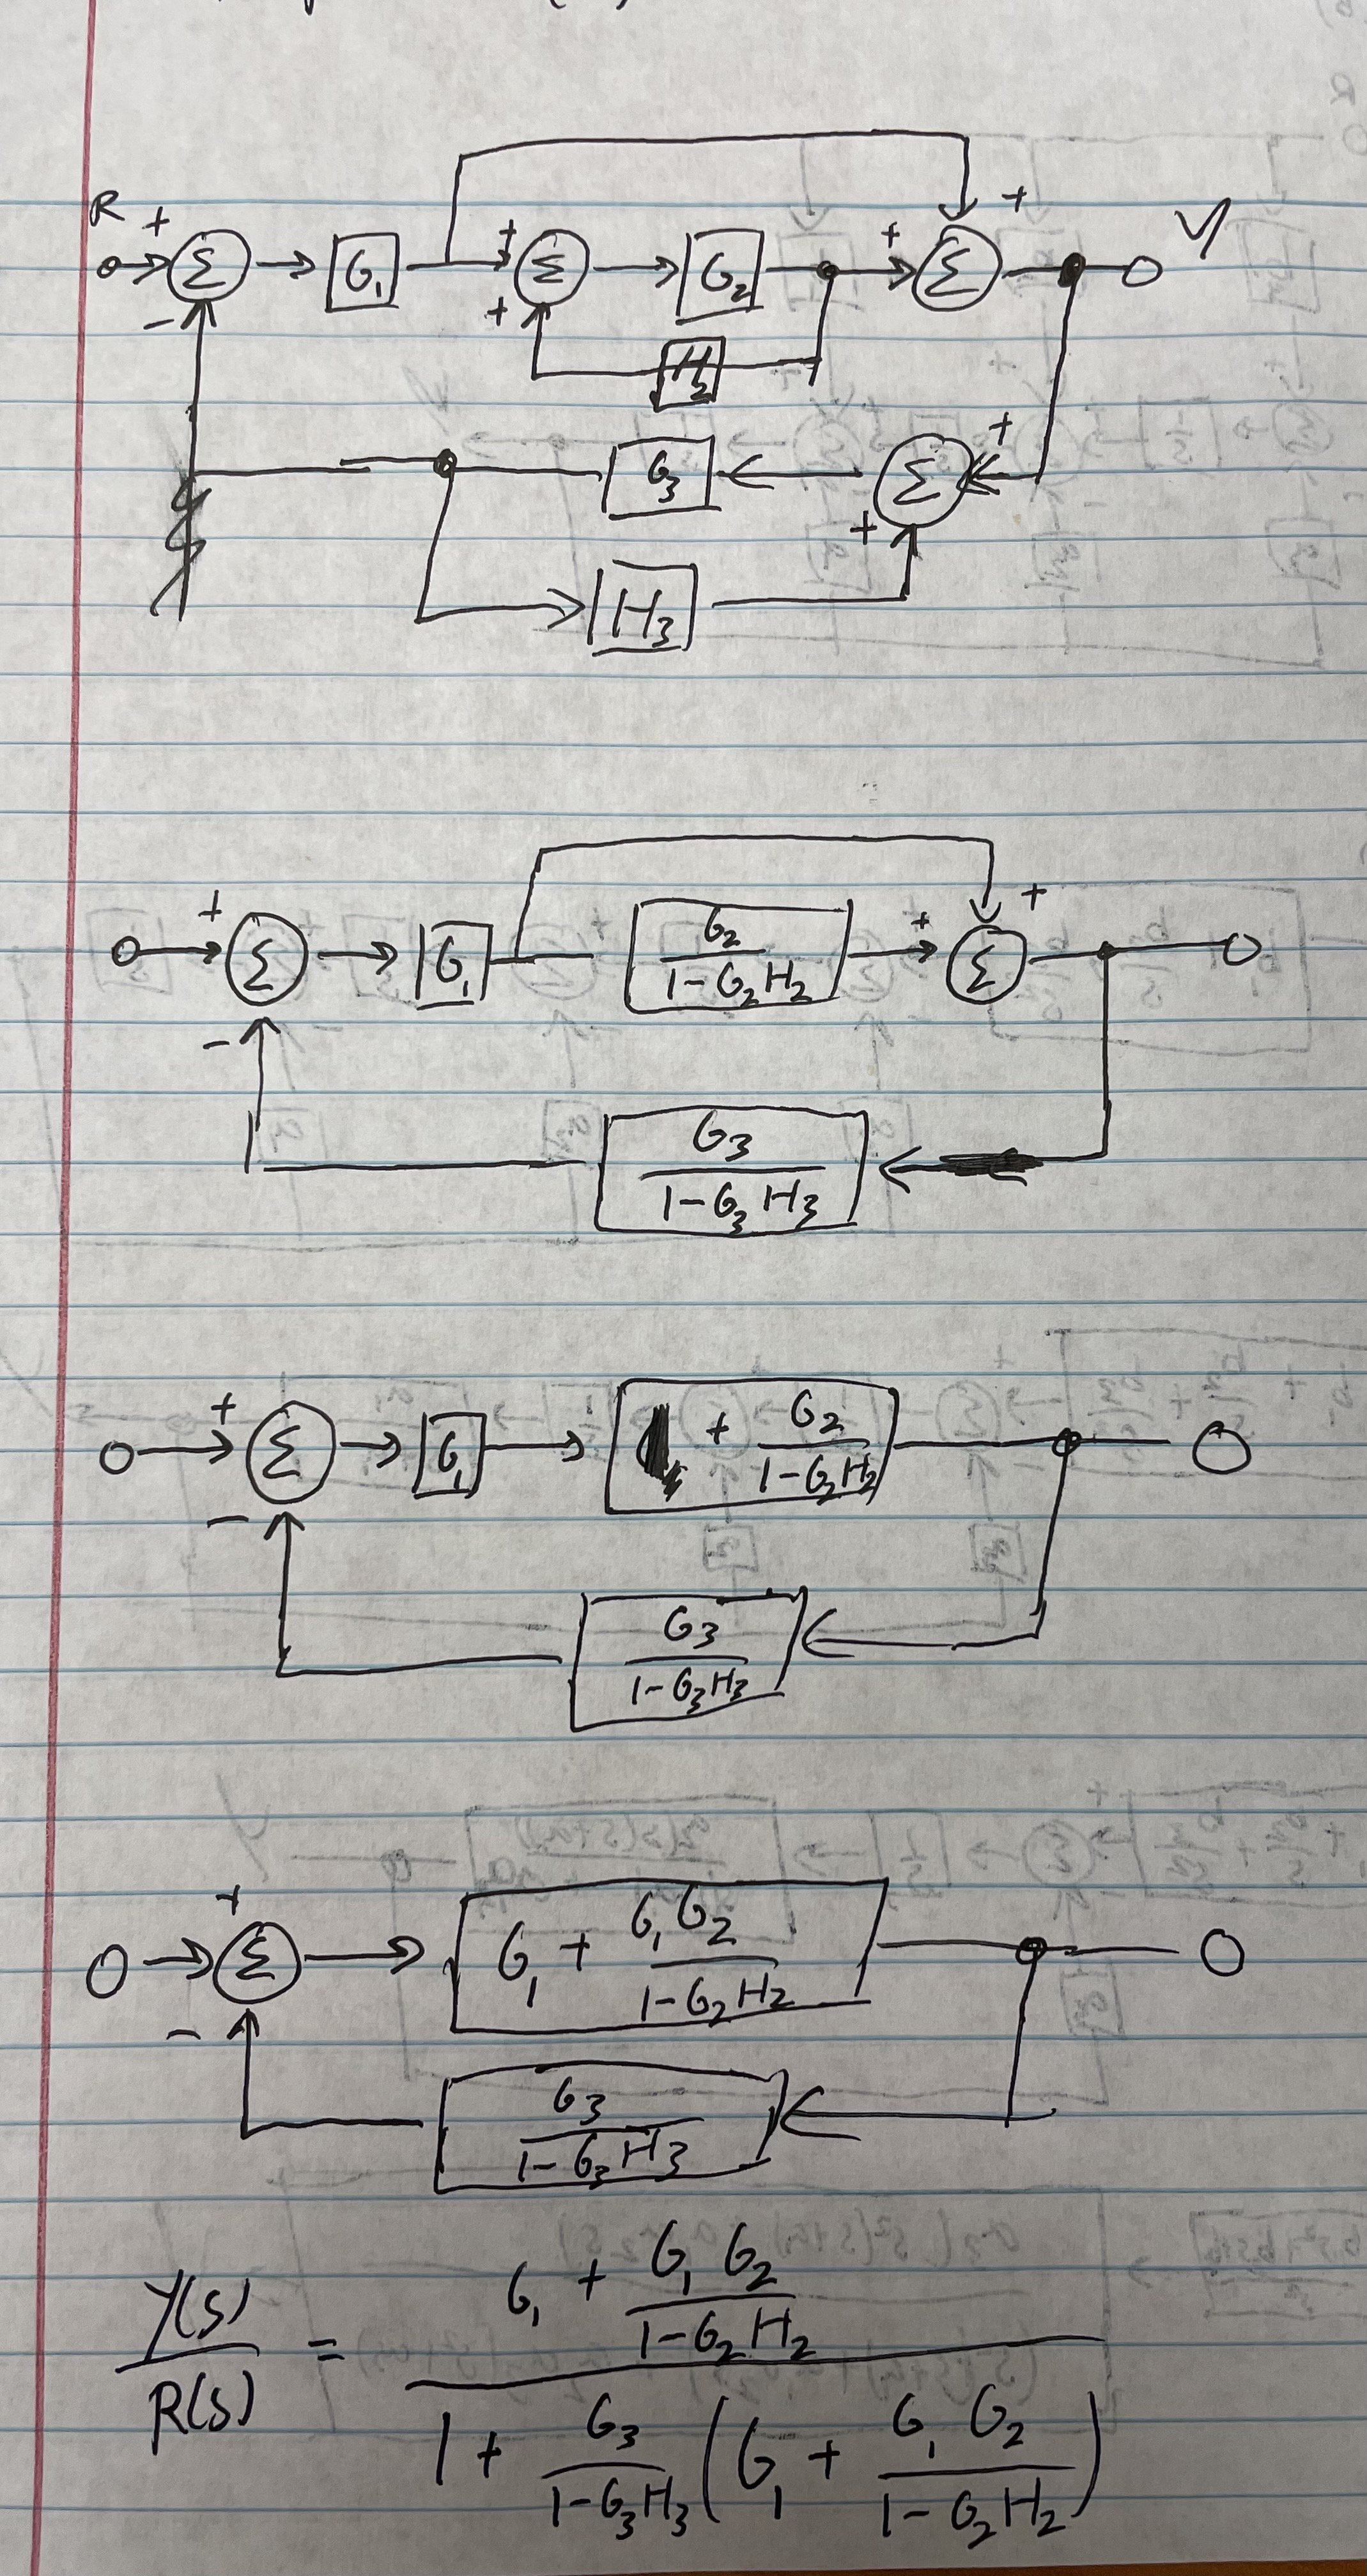
\includegraphics[scale=0.1]{Problem1a.JPG}
\FloatBarrier
$$\frac{Y(s)}{R(s)}=\frac{G_1+\frac{G_1G_2}{1-G_2H_2}}{1+\left(G_1+\frac{G_1G_2}{1-G_2H_2}\right)\frac{G_3}{1-G_3H_3}}$$

\subsection*{(b)}
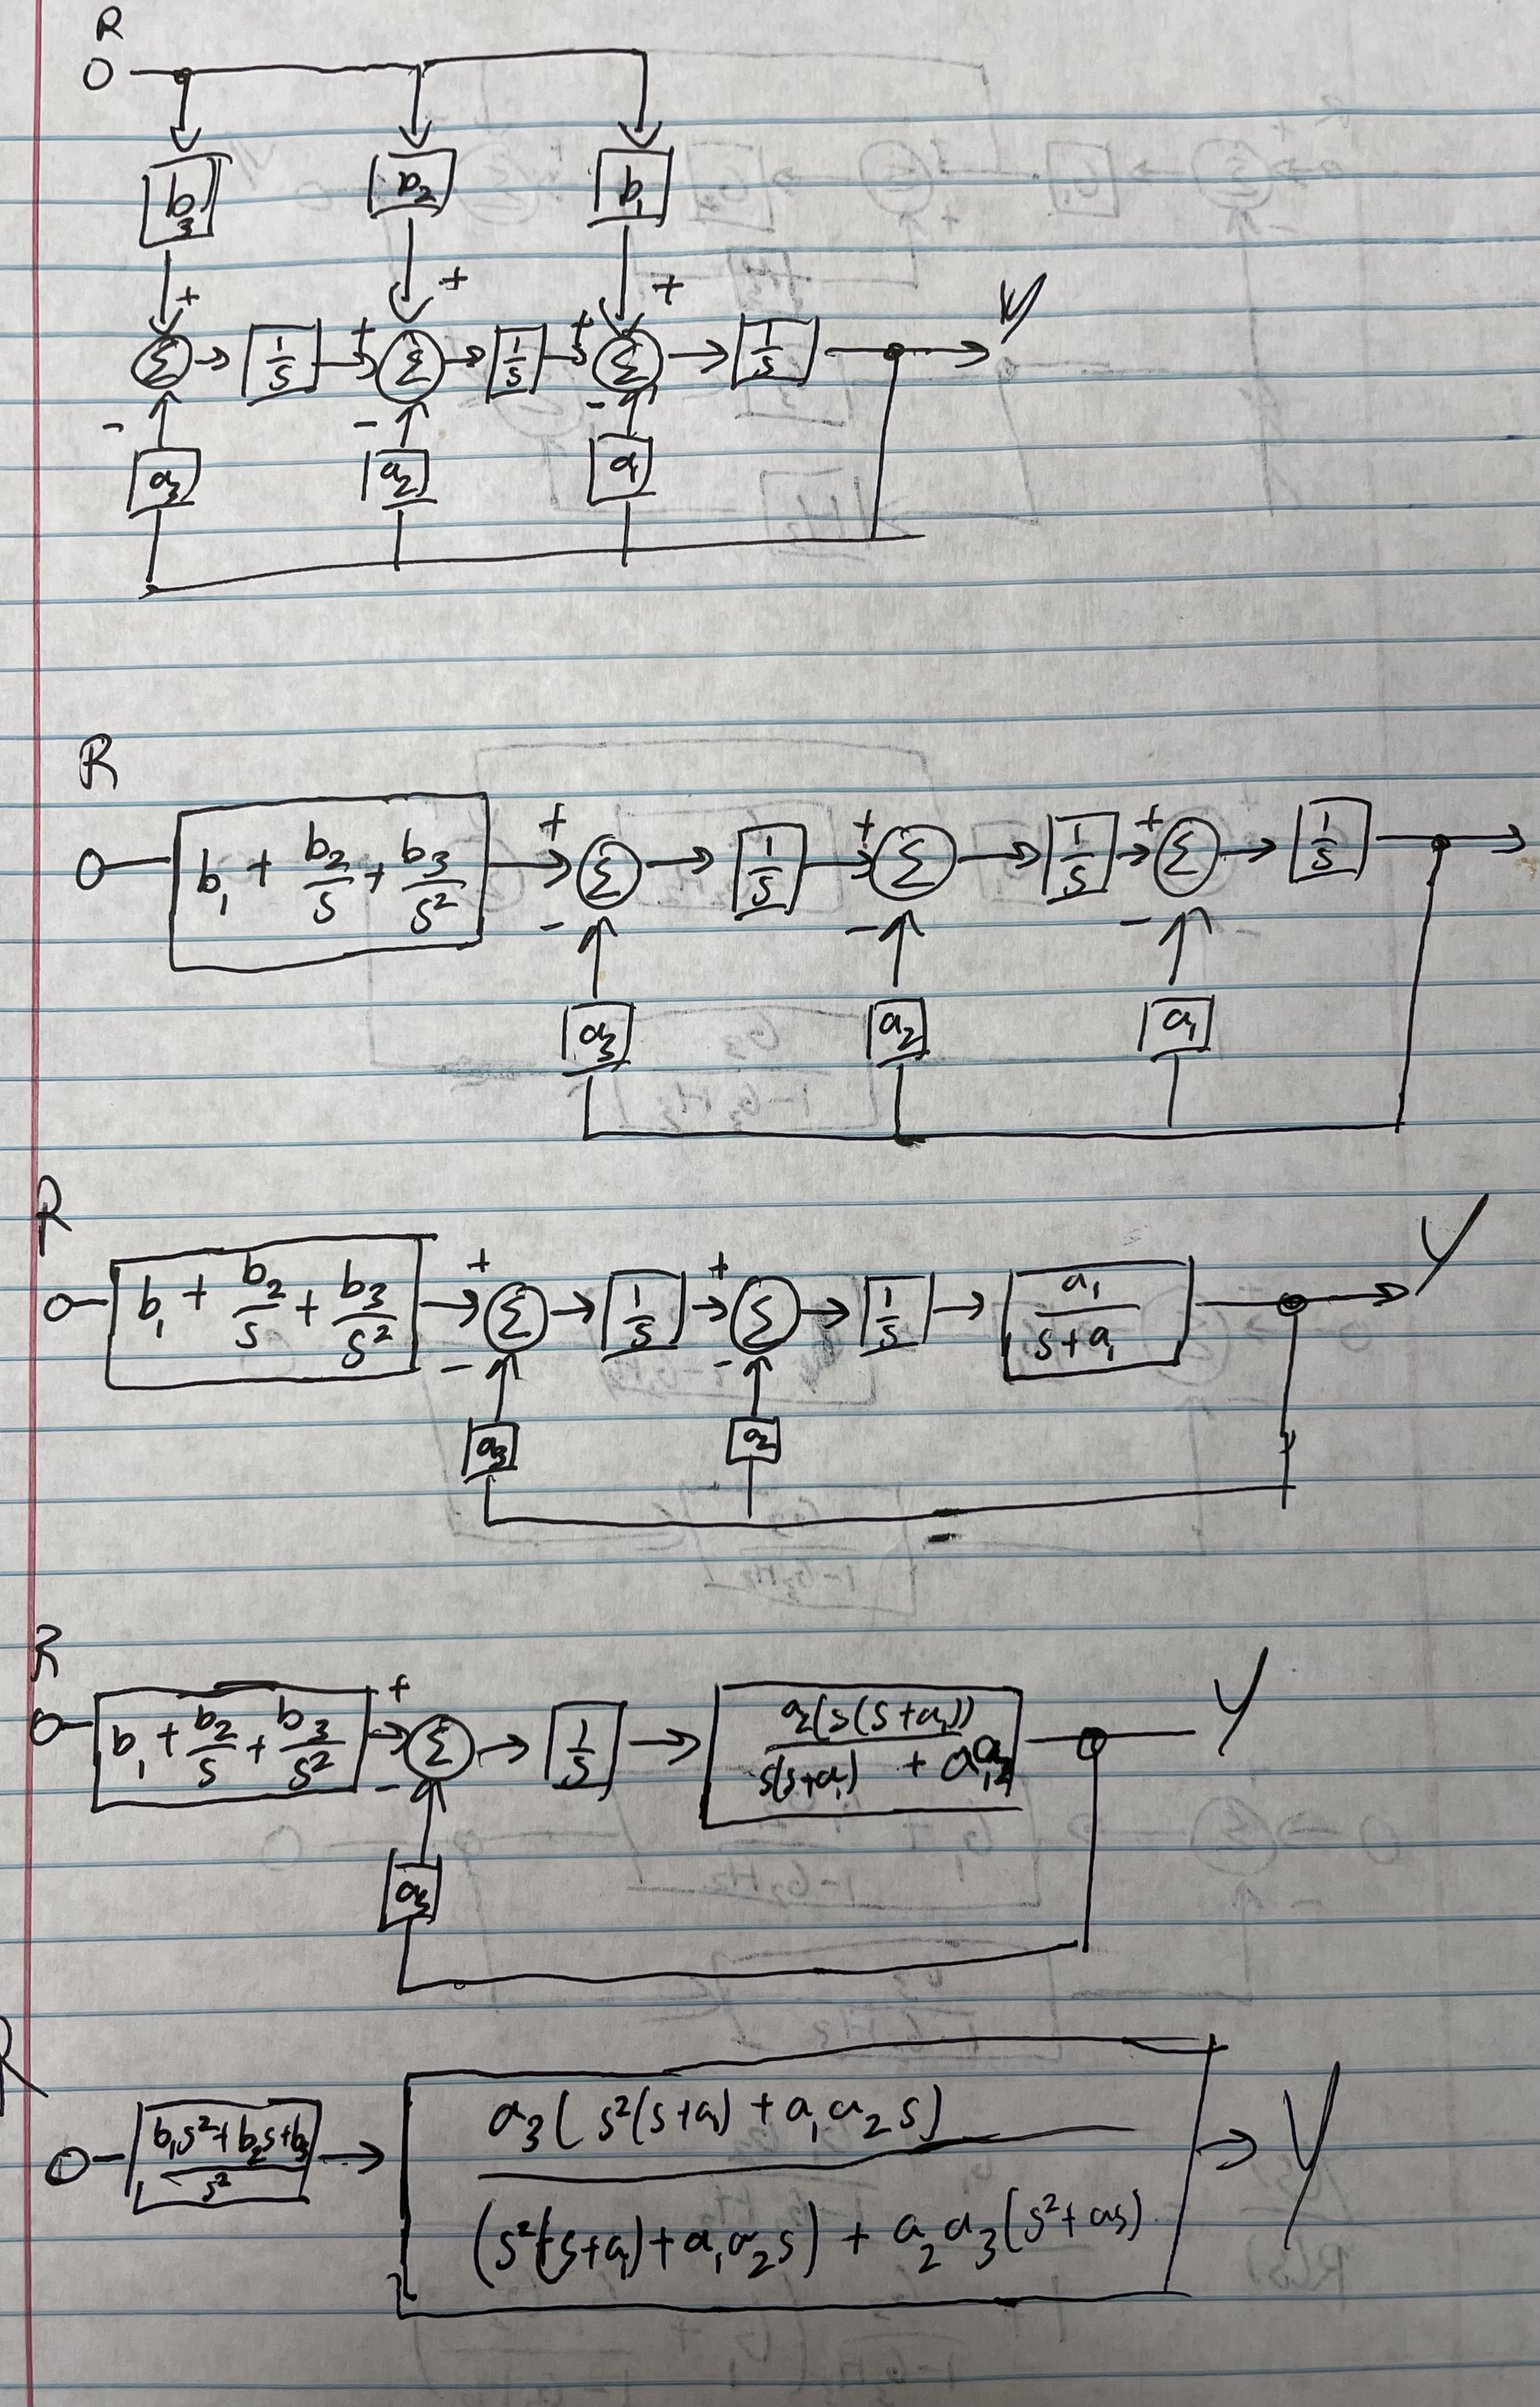
\includegraphics[scale=0.5]{Problem1b.JPG}
\FloatBarrier
$$\frac{Y(s)}{R(s)}=\boxed{\frac{b_1s^2+b_2s+b_3}{s^2}+
\frac{a_3(s^2(s+a_1)+a_1a_2s)}{s^2(s+a_1)+a_1a_2s+a_2a_3(s^2+a_1s)}}$$

\subsection*{(c)}
\includegraphics[scale=0.5,angle=270,origin=c]{Problem1c.JPG}
\FloatBarrier
$$\frac{Y(s)}{R(s)}=\boxed{\frac{b_1s^2+b_2s+b_3}{s^3+a_1s^2+a_2s+a_3}}$$
\subsection*{(d)}
\includegraphics[scale=0.5,angle=270,origin=c]{Problem1d.JPG}
\FloatBarrier
$$\frac{Y(s)}{R(s)}=\boxed{\frac{D(s)+D(s)B(s)H(s)+A(s)B(s)}
{1+B(s)H(s)+G(s)(D(s)+D(s)B(s)H(s)+A(s)B(s))}}$$
\section*{Problem 3.30}
\subsection*{(a)}
We have
$$16\%\geq M_p=e^{-\pi\frac{\zeta}{\sqrt{1-\zeta^2}}}$$
$$6.9\geq t_s=\frac{4.6}{\zeta \omega_n}$$
$$1.8\geq t_r=\frac{1.8}{\omega_n}$$
Therefore we get three conditions
$$\omega_n\geq1$$
$$\sigma\leq-\frac{4.6}{6.9}$$
$$\sin^-1(\zeta)\leq\tan^{-1}\frac{-\ln(0.16)}{\pi}$$
From these we get the following region

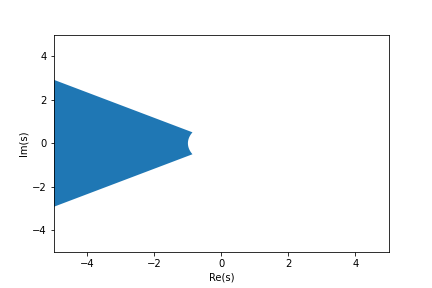
\includegraphics[scale=.5]{Problem2.png}
\FloatBarrier
\section*{(b)}
We therefore have
$$1.8=t_r=\frac{1.8}{\omega_n}$$
Therefore $\omega_n=1$, furthermore we have
$$6.9=t_r=\frac{4.6}{\zeta \omega_n}=\frac{4.6}{\zeta}$$
Therefore $\zeta=\frac{4.6}{6.9}=\frac{2}{3}$ and thus we have that the overshoot
$$M_p=e^{-\pi \frac{2}{\sqrt{5}}}$$
$$M_p=6\%$$
\section*{Problem 3.32}
\subsection*{(a)}
Therefore we have that the transfer function is 
\begin{align*}
    \frac{Y(s)}{R(s)}&=\frac{G(s)}{1+G(s)}\\
    &=\frac{K}{s^2+2s+K}
\end{align*}
Therefore we have
$$K=\omega_n^2$$
$$\zeta\omega_n=1$$
Furthermore from the peak time and overshoot criterion we have
$$t_p=\frac{\pi}{\omega_d}=\frac{\pi}{\omega_n\sqrt{1-\zeta^2}}=1$$
$$M_p=e^{-\pi\frac{\zeta}{\sqrt{1-\zeta^2}}}=0.05$$
Using the equation from $t_p$ and applying $\omega_n=\frac{1}{\zeta}$ we have
$$\frac{\pi\zeta}{\sqrt{1-\zeta^2}}=1$$
$$\frac{\zeta}{\sqrt{1-\zeta^2}}=\frac{1}{\pi}$$
Plugging this into $M_p$ we get
$$e^{-\pi\frac{1}{\pi}}=0.367\neq0.05$$
Therefore we cannot meet both specifications just by selecting
the right value of $K$
\subsection*{(b)}
From the peak time and overshot criterion we have
$$\omega_n\sqrt{1-\zeta^2}=\pi$$
and
$$\omega_n\zeta=-\ln(0.05)$$

Therefore we have poles at 
$$s=\ln(0.05)\pm \pi j$$
Furthermore, the poles for $\frac{Y(s)}{R(s)}$ are at 
$$s=\frac{-2\pm\sqrt{4-4K}}{2}=-1\pm\sqrt{1-K}$$
Therefore we get the following sketch for the poles in the s plane 

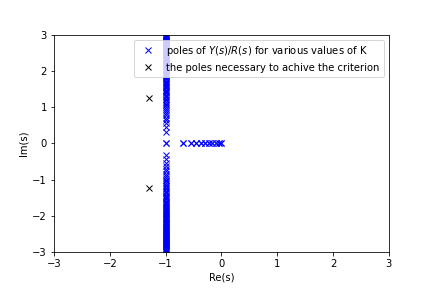
\includegraphics[scale=.5]{Problem3}
\FloatBarrier
\subsection*{(c)}
We relax the conditions by multiplying the peak time
and overshoot with $c$ therefore we have
$$t_p=\frac{\pi}{\omega_n\sqrt{1-\zeta^2}}=c$$
$$M_p=e^{-\pi\frac{\zeta}{\sqrt{1-\zeta^2}}}=0.05c$$
thererfore since $\omega_n=\frac{1}{\zeta}$

$$\frac{\zeta}{\sqrt{1-\zeta^2}}=\frac{c}{\pi}$$
therefore we have
$$-c=\ln(0.05)+\ln(c)$$
Solving this we have
$$c=2.205$$
$$M_P=11\%$$
$$t_p=2.205s$$
And therefore we have
$$\frac{1}{\sqrt{\omega_n^2-1}}=\frac{c}{\pi}=0.701$$
therefore we have
$$\frac{1}{0.701^2}=\omega_n^2-1$$
$$K=\omega_n^2=\frac{1}{0.701^2}+1=3.034$$


\section*{Problem 3.36}
\subsection*{(a)}
Applying the laplace transform we get
$$Js^2\Theta(s)+Bs\Theta(s)=T_c(s)$$
$$\frac{\Theta(s)}{T_c(s)}=\boxed{\frac{1}{Js^2+Bs}}$$
\subsection*{(b)}
Therefore we have
$$J\theta''+B\theta'=K(\theta_r-\theta)$$
$$Js^2\Theta(s)+Bs\Theta(s)+K\Theta(s)=K\Theta_r(s)$$
$$\frac{\Theta_r(s)}{\Theta(s)}=\boxed{\frac{K}{Js^2+Bs+K}}$$
\subsection*{(c)}
For overshoot we have
$$M_p=e^{-\pi\frac{\zeta}{\sqrt{1-\zeta^2}}}<0.1$$
$$-\pi\frac{\zeta}{\sqrt{1-\zeta^2}}<\ln(0.1)$$
$$-\pi\zeta<\ln(0.1)\sqrt{1-\zeta^2}$$
$$\pi^2\zeta^2>\ln^2(0.1)(1-\zeta^2)$$
$$(\pi^2+\ln^2(0.1))\zeta^2>\ln^2(0.1)$$
$$\zeta>\sqrt{\frac{\ln^2(0.1)}{\pi^2+\ln^2(0.1)}}$$
And since 
$$\zeta\omega_n=\frac{B}{2J}$$
We have
$$\omega_n=\frac{B}{2\zeta}<\frac{B}{2J}\sqrt{\frac{\pi^2+\ln^2(0.1)}{\ln^2(0.1)}}$$
And since
$$\omega_n^2=\frac{K}{J}$$
We have
$$\frac{K}{J}<\frac{B^2}{4J^2}\frac{\pi^2+\ln^2(0.1)}{\ln^2(0.1)}$$
$$K<\frac{B^2}{4J}\frac{\pi^2+\ln^2(0.1)}{\ln^2(0.1)}$$
$$K<476.92$$
\subsection*{(d)}
In order for the rise time to be less than 80 seconds we must have
$$t_p=\frac{1.8}{\omega_n}<80$$
$$\frac{1.8}{80}<\omega_n$$
and since we have $\omega_n^2=\frac{K}{J}$ we have
$$\frac{1.8^2}{80^2}J<K$$
$$K>\boxed{303.75}$$


\end{document}
